\documentclass{standalone}
\usepackage{tikz}
\usetikzlibrary{arrows.meta, positioning}

\begin{document}
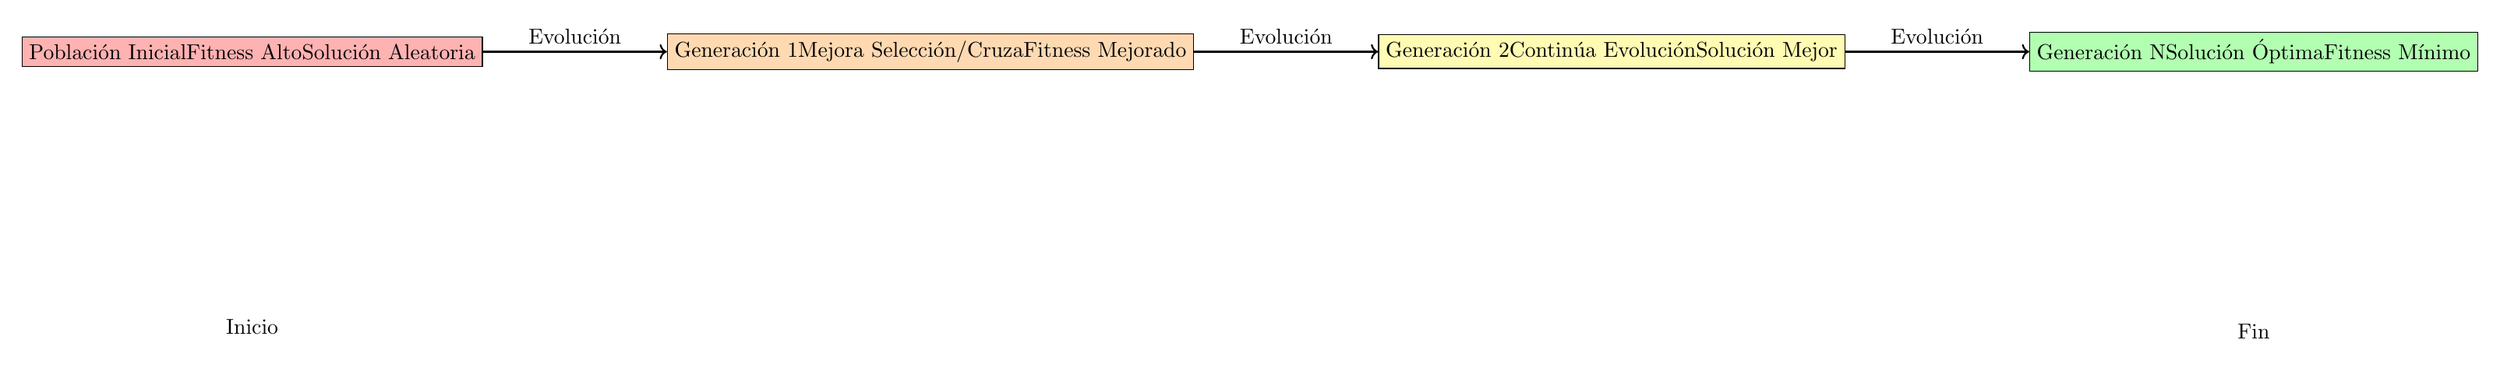
\begin{tikzpicture}[node distance=3cm]
    % Definir nodos para generaciones
    \node (gen0) [draw, rectangle, fill=red!30, minimum width=3cm] {Población Inicial\\Fitness Alto\\Solución Aleatoria};
    \node (gen1) [draw, rectangle, fill=orange!30, right=of gen0, minimum width=3cm] {Generación 1\\Mejora Selección/Cruza\\Fitness Mejorado};
    \node (gen2) [draw, rectangle, fill=yellow!30, right=of gen1, minimum width=3cm] {Generación 2\\Continúa Evolución\\Solución Mejor};
    \node (genn) [draw, rectangle, fill=green!30, right=of gen2, minimum width=3cm] {Generación N\\Solución Óptima\\Fitness Mínimo};

    % Dibujar flechas de evolución
    \draw[->, thick] (gen0) -- (gen1) node[midway, above] {Evolución};
    \draw[->, thick] (gen1) -- (gen2) node[midway, above] {Evolución};
    \draw[->, thick] (gen2) -- (genn) node[midway, above] {Evolución};

    % Añadir indicador de mejora
    \node [below=of gen0, yshift=-1cm] {Inicio};
    \node [below=of genn, yshift=-1cm] {Fin};
\end{tikzpicture}
\end{document}